

Attention now turns to the assessment of ASV vulnerabilities.  With a strictly controlled protocol, the potential impact of replay attacks is compared to that of speech synthesis and voice conversion.  It is stressed that the experiments do not and cannot evaluate every possible replay scenario in exhaustive fashion; the aim is simply to gauge the relative threat and the potential to detect attacks with dedicated countermeasures. 


\subsection{Replay spoofing}

\begin{figure}
	\centering
	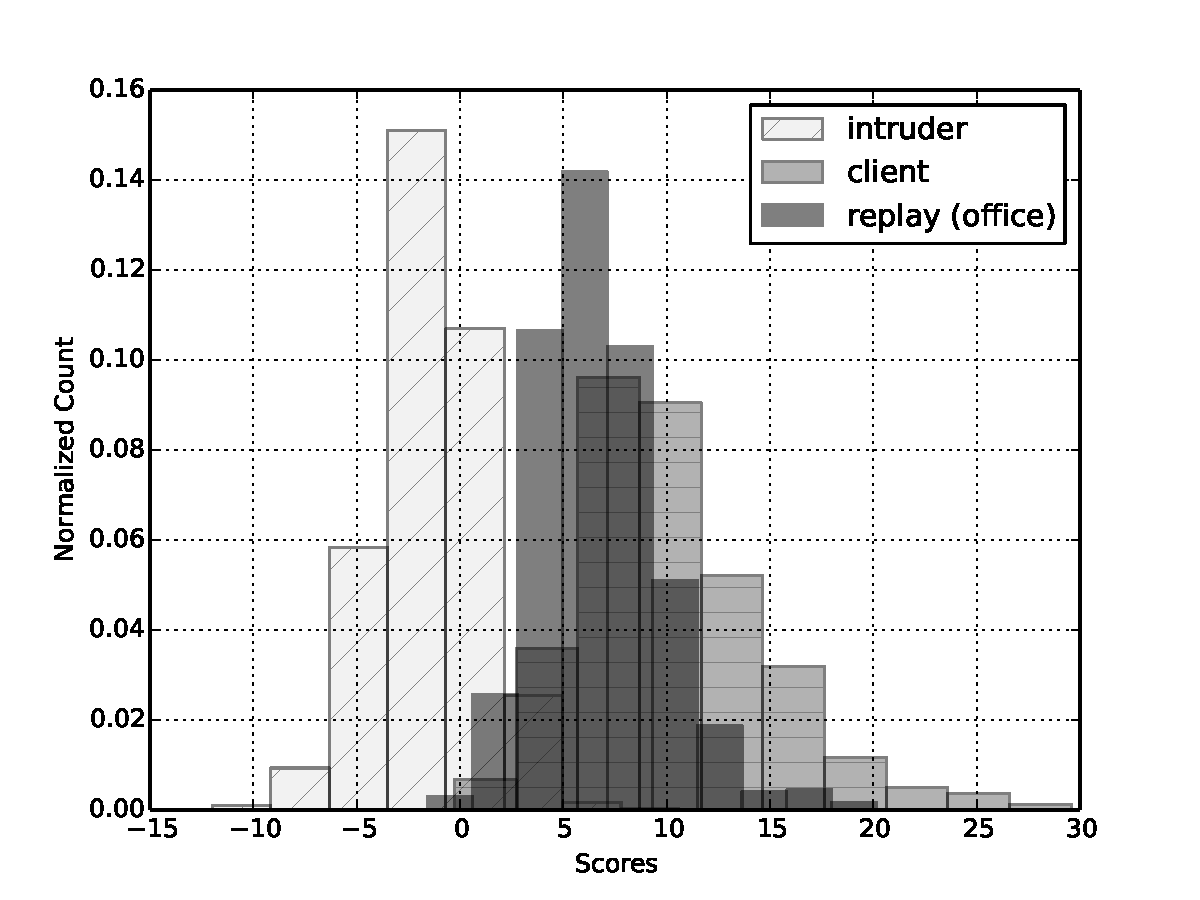
\includegraphics[width=1\linewidth]{Figs/dist_IV_off.pdf}
	\caption{Score distribution for the IV-PLDA system for replay attacks using an emulated high-quality speaker and an office environment.}
	\label{fig::Dist_IV}
\end{figure}


% distributions
Fig.~\ref{fig::Dist_IV} shows the effect of replay attacks on the score distributions for the IV-PLDA system.  Replay attacks correspond to an emulated high-quality speaker and office environment.  Three distributions are illustrated: (i) the zero-effort impostor distribution; (ii) the genuine client distribution, and (iii) the distribution obtained when all zero-effort impostor trials are replaced with replay attacks.  While the zero-effort impostor and genuine client distributions are well separated, the latter overlaps significantly with the score distribution for replay attacks.  Increased overlap between these distribution will degrade ASV performance.



\begin{table*}
\renewcommand{\arraystretch}{1.2}
\begin{center}
%    \begin{tabular}{ l l || c c c c c c c}
    \begin{tabular}{ l  c c c c c c c}
    \hline
%Score norm & Replay env. &  GMM & SGL & SGL-NAP  & SGL-FA & FA & IV & IV-PLDA \\ 
 &  GMM & SGL & SGL-NAP  & SGL-FA & FA & IV & IV-PLDA \\ 
 \hline \hline
%& (Baseline) & 9.08 & 7.89 & 6.35 & 6.08 & 5.60 & 6.67 & 3.20\\
%No & Office  & 40.26 & 34.43 & 33.52 & 30.72 & 33.85 & 27.83 & 29.11\\
%norm & Corridor & 35.71 & 28.24 & 28.53 & 25.75 & 29.92 & 23.02 & 22.78\\
%& None & 51.59 & 49.64 & 49.49 & 49.73 & 49.37 & 49.38 & 49.37\\
%\hline
%& (Baseline) & 8.63 & 8.13 & 6.31 & 5.72 & 5.61 & 6.72 & 2.98\\
%With & Office  & 60.32 & 92.98 & 29.92 & 28.54 & 30.12 & 28.89 & 30.30\\
%norm & Corridor & 55.91 & 88.20 & 23.59 & 21.62 & 24.97 & 23.31 & 24.53\\
%& None & 64.40 & 96.67 & 49.44 & 49.31 & 49.67 & 49.06 & 49.46\\
Baseline & 8.63 & 8.13 & 6.31 & 5.72 & 5.61 & 6.72 & 2.98\\
\hline
Replay: office environment & 60.32 & 92.98 & 29.92 & 28.54 & 30.12 & 28.89 & 30.30\\
Replay: corridor environment & 55.91 & 88.20 & 23.59 & 21.62 & 24.97 & 23.31 & 24.53\\
Replay: anechoic environment & 64.40 & 96.67 & 49.44 & 49.31 & 49.67 & 49.06 & 49.46\\
\hline
Voice conversion & 33.69 & 36.92 & 27.58 & 23.97 & 23.96 & tbc. & 19.30\\
Speech synthesis & 27.29 & 15.04 & 13.78 & 11.91 & 16.22 & tbc. & 10.82\\
\hline
    \end{tabular}
%    \caption{EER values for different ASV systems for various acoustic %environment of replay attacks, with and without score normalisation. }
    \caption{Equal error rates (EERs) for seven different ASV systems and for zero-effort impostors (baseline) and three different replay attack configurations (three different acoustic environments).  Results are averaged across the three different loudspeaker configurations.}
		\label{tab::results_EER}
   \end{center}

\end{table*}


\begin{figure}[!t]
	\centering
	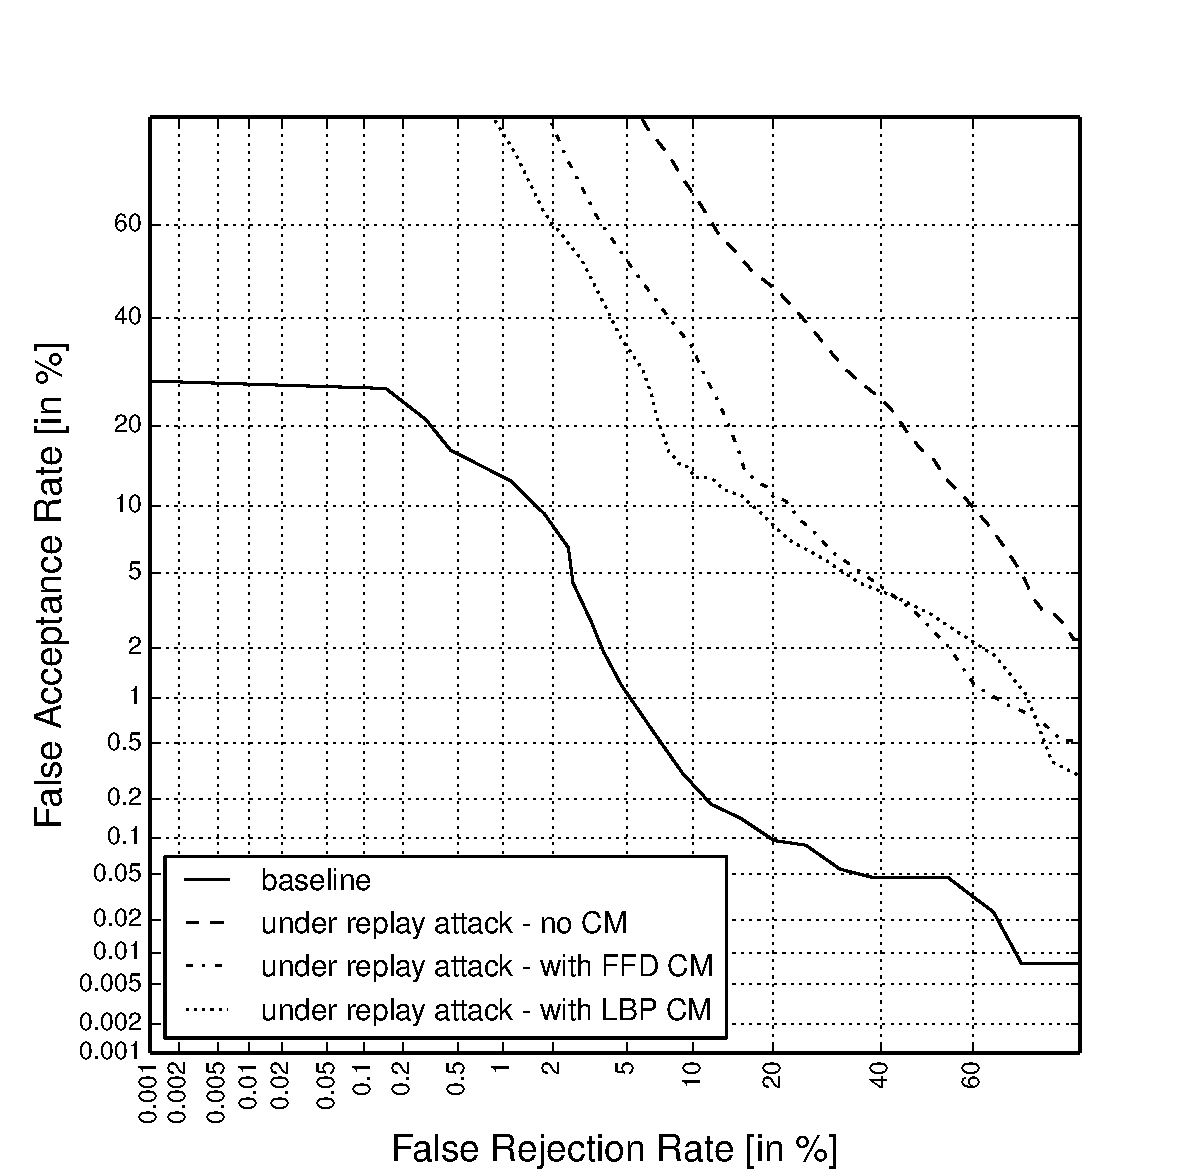
\includegraphics[width=1\linewidth]{Figs/DET_IVPLDA_counter_Behr.pdf}
	\caption{DET plots for the IV-PLDA system: (i) the baseline, (ii) under replay spoofing with a high-quality speaker in an office, (iii) under replay attack, but with FFD and (iv) LBP countermeasures.}

%% {\bfseries There is too much information on this plot.  I suggest to include only four profiles: (i) the baseline, (ii) spoofing under the same conditions as in Fig.~\ref{fig::Dist_IV} and (iii) and (iv) with FFD and LBP countermeasures - to be referred to later.}}
	\label{fig::DETs_replay_IV}
\end{figure}


% DET plots
Fig.~\ref{fig::DETs_replay_IV} illustrates a detection error trade-off (DET) plot\footnote{The DET plots were produced with the TABULA RASA Scoretoolkit (http://publications.idiap.ch/downolads/reports/2012/Anjos\_Idiap-Com-02-2012.pdf).} for the same experimental setup.  The lower-most, solid profile illustrates the performance of the baseline ASV system.  The upper-most, dashed profile illustrates performance when zero-effort impostors are replaced with replay attacks.  The difference between these two profiles thus serves as an indication of system vulnerability to replay spoofing; in this case the degradation in performance is significant.  



% EER table described
This trend is observed across the full set of seven ASV systems and nine different replay attack configurations;  
results are illustrated in Table~\ref{tab::results_EER}.
Results in the second row show the baseline performance for each ASV system and for only zero-effort impostors.
As expected, the IV-PLDA system delivers the lowest EER.
Rows 2--5 illustrate the degradation in performance when zero-effort impostors are replaced with replay attacks applied in three different acoustic environments.
EERs in Table~\ref{tab::results_EER} are averaged across the three loudspeaker configurations; other results not reported here showed greater sensitivity to the acoustic environment than to the loudspeaker characteristics.  
The performance of all seven systems degrades significantly.
The EER of the most sensitive GSL system increases from 8\% to approximately 90\% for all three acoustic environments. We suspect that such a strong degradation is an unwanted effect of score normalisation based on the T-norm algorithm, however this hypothesis requires further investigation.
Even the EER of the most resistant SGL-FA system increases to between 22\% and 50\%.  
Finally, the EER of the state-of-the-art IV-PLDA system increases to between 25\% and 50\%.  Even discounting the anechoic environment, the EER is as high as 30\%.


%% comparison with other attacks
\subsection{Comparison to voice conversion and speech synthesis}

\begin{figure}[!t]
	\centering
	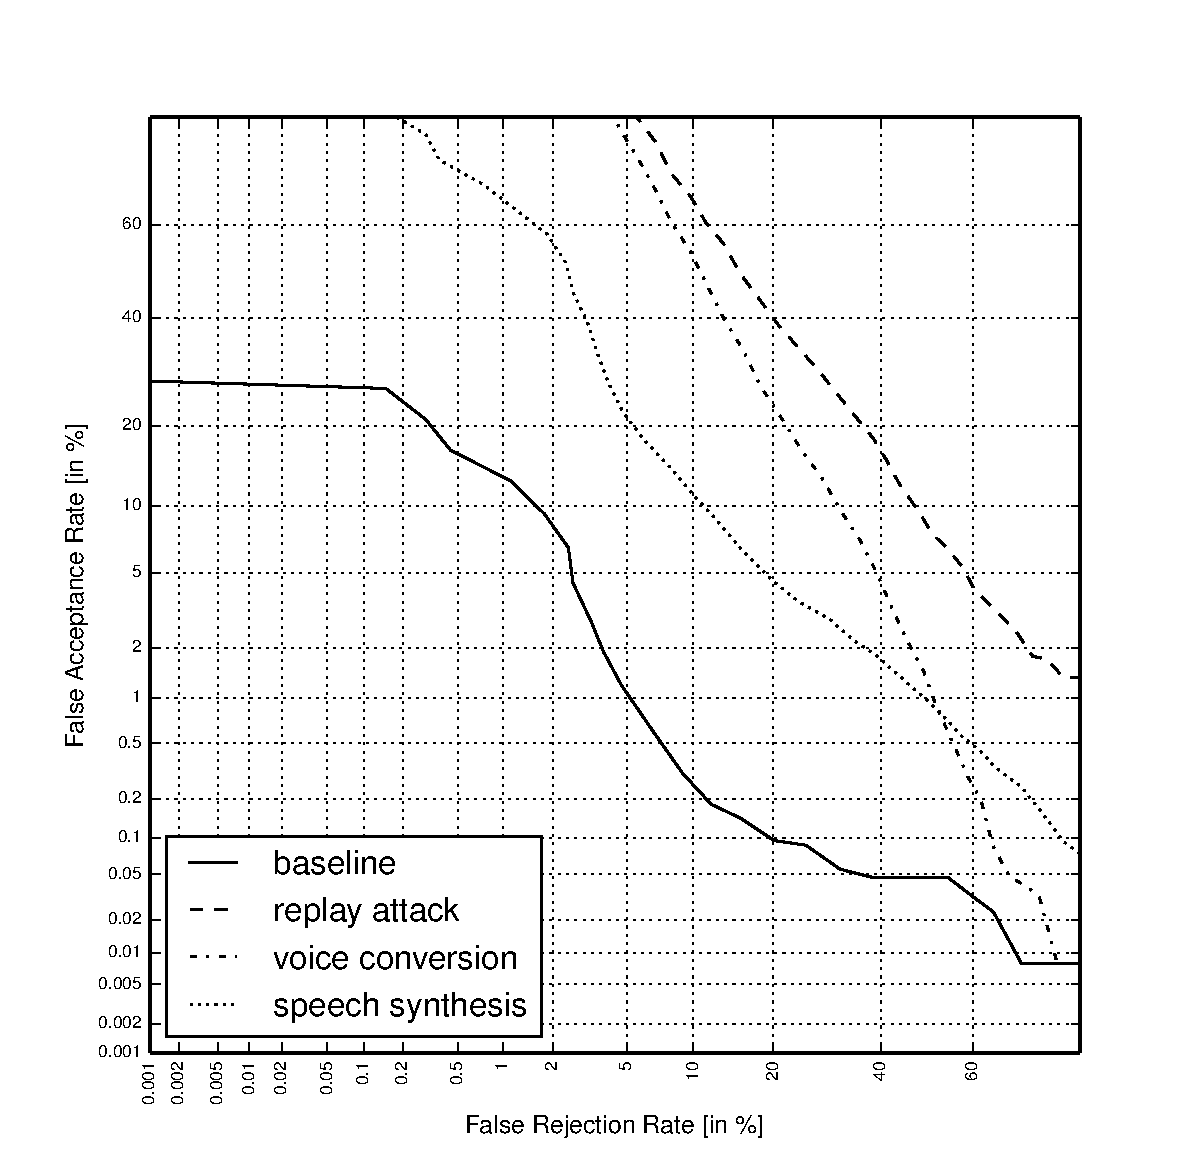
\includegraphics[width=1\linewidth]{Figs/DETs_IV_ss_vc_rp.pdf}
	\caption{DET plots for iVector-PLDA system and various attacks.}
% {\bfseries Axis keys and labels are too small.}}
	\label{fig::DETs_4attacks}
\end{figure}

DET profiles showing the comparative vulnerabilities to replay, voice conversion and speech synthesis attacks are illustrated in Fig.~\ref{fig::DETs_4attacks} for the IV-PLDA system.  While the comparison of such profiles is not strictly meaningful\footnote{Different spoofing algorithms will yield different degradations in ASV performance.  For example, other authors~\cite{DeLeon2012}, show considerably greater vulnerabilities for speech synthesis.} it is clear that it is a mistake to discount the threat of replay attacks.  This trend is consistent across the full range of ASV systems.  Again, while the comparisons are not strictly meaningful, being sufficient only to gauge the relative threat, results in rows 6 and 7 of Tab.~\ref{tab::results_EER} show the broad vulnerability of all seven ASV systems to replay attacks.





\subsection{Replay countermeasure}


\begin{table*}
\renewcommand{\arraystretch}{1.2}
\begin{center}
    \begin{tabular}{ l || c c c | c c c}
    \hline
 \multirow{2}{*}{Environment}  & \multicolumn{3}{c|}{EER (\%)} & \multicolumn{3}{c}{SFAR (\%)} \\
     	 & no CM & with FFD & with LBP & no CM & with FFD & with LBP\\ 

 \hline \hline
Office   & 30.30 & 13.62 & 9.56 & 88.70 & 63.93 & 46.29\\
Corridor & 24.53 & 11.34 & 7.00 & 80.91 & 50.25 & 30.52\\
None & 49.46 & 42.14 & 46.77 & 97.00 & 95.17 & 95.76\\
\hline
    \end{tabular}
    \caption{EER and SFAR values for various environment of replay attacks, with and without the FFD or LBP countermeasures applied, for IV-PLDA. The SFAR was measured for FRR equal to the baseline EER (2.98\%).}
		\label{tab::results_CM_rooms}
   \end{center}
\end{table*}




Fig.~\ref{fig::DETs_CM} illustrates (independently of ASV) the performance of the far-field (FFD) and local binary pattern (LBP) countermeasures in detecting replay attacks.  Results are illustrated for emulated attacks using a high-quality loudspeaker and averaged across both office and corridor environments.  
Results show that the LBP countermeasure yields considerably better results than the FFD countermeasure (EERs of 2.87\% and 16.53\% respectively).  Since no far-field effects were included in the replay emulation, it is perhaps not surprising that FFD countermeasure performance is relatively poor.  Note also the step-like nature of the DET curve for the LBP countermeasure which is typical in the case of classifiers based on decision trees, as the AdaBoost
M1 classifier used in this project.


The middle two profiles in Fig.~\ref{fig::DETs_replay_IV} show the impact of each countermeasure when integrated with the IV-PLDA ASV system.  %We selected this ASV, since it is the state-of-the-art, widely used ASV solution, and therefore it is likely that it can be a victim of replay spoofing. The middle two profiles in Fig.~\ref{fig::DETs_replay_IV} show the impact of the far-field detection and LBP-based countermeasures on such a system. 
While both countermeasures show reductions in the EER compared to the upper-most profile, performance still remains far from the baseline.


Detailed results for FFD and LBP countermeasures and three replay environments are presented in Table~\ref{tab::results_CM_rooms}.  Results are again averaged for the three different loudspeakers and are presented in terms of both EER and SFAR.  Unsurprisingly, results for the anechoic environment show that neither countermeasure performs well.  Consistent to results in Fig.~\ref{fig::DETs_replay_IV}, the LBP countermeasure again outperforms the FFD countermeasure.  While replay in office and corridor environments leads to significant degradations in ASV performance, EERs with active countermeasures are less than 10\%.  Even so, they remain high.  Even if the reduction in equivalent SFAR results is significant, even with active countermeasures the SFAR remains no lower than 30\%.  These results suggest that replay spoofing is far from a solved problem. %the situation is concerning;  than replay in a corridor environment, the realtive improvement  The relative improvement caused by the countermeasures turned out to be the highest for the office -- in this case the EER decreased from 30\% down to less than 14\% for FFD and less than 10\% for LBP. Also for the corridor LBP turned out to be more effective than FFD -- 7\% EER vs. 11\%, respectively, also the SFAR result was much lower (30\% vs. 46\%). When acoustic conditions were not considered, both countermeasures performed poorly, with the EER results slightly better for FFD. 



%% DETs w/wo CM
\begin{figure}
	\centering
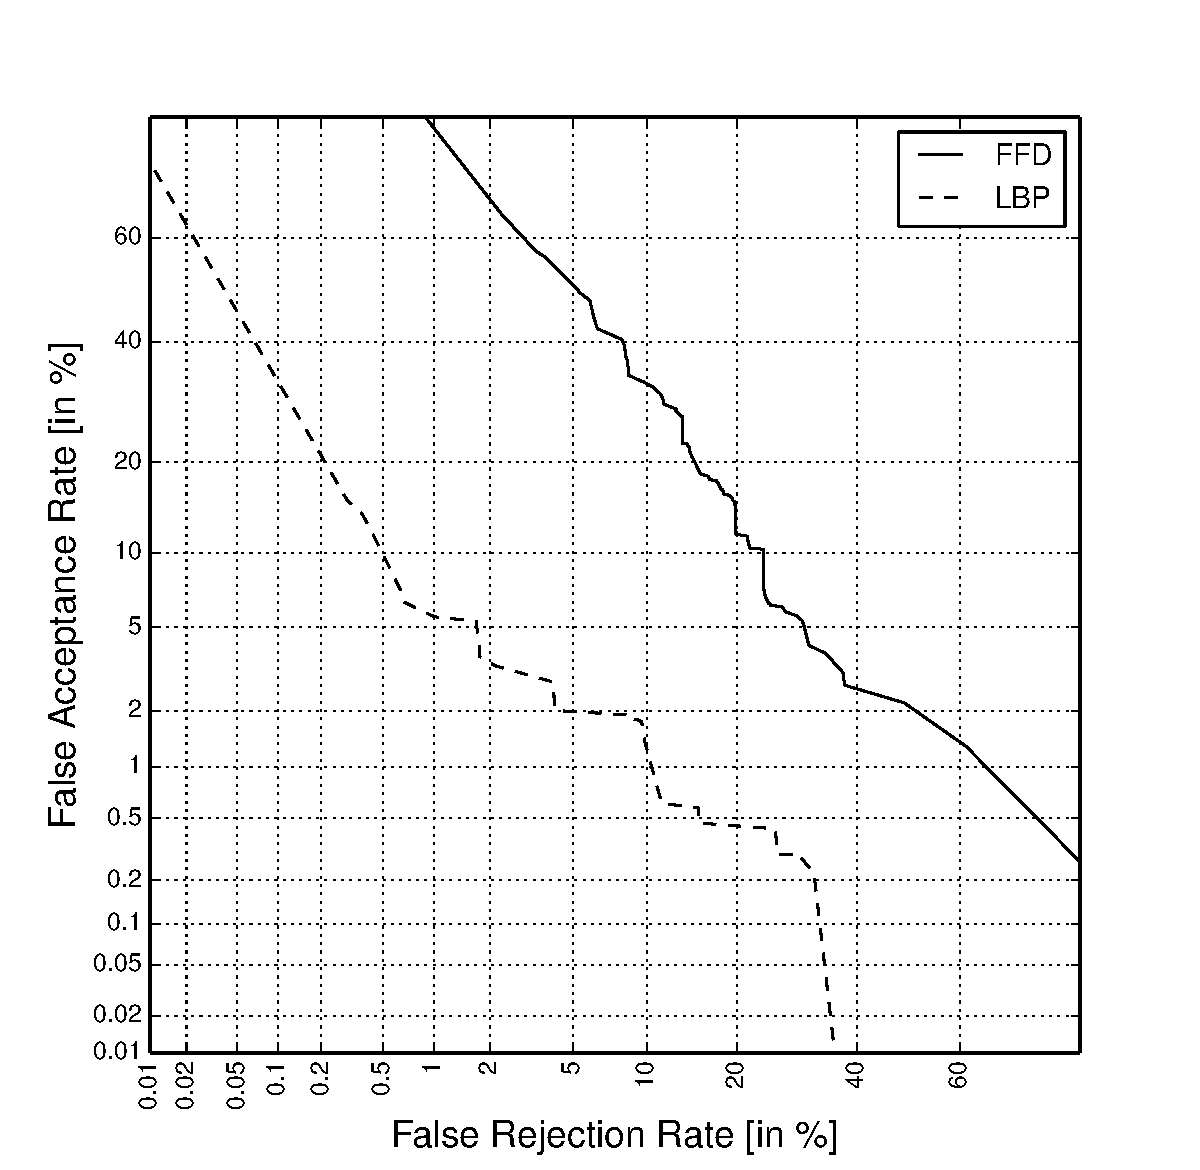
\includegraphics[width=1\linewidth]{Figs/DET_CM.pdf}
	\caption{DET plots for replay spoofing detection using the FFD or LBP countermeasures (assessment independent from ASV), for a high-quality speaker.}
	\label{fig::DETs_CM}
\end{figure}



% discussion 
\subsection{Interpretation of results}

The results presented above corroborate the findings of previous work performed with considerably smaller databases; unsurprisingly, replay attacks represent a tangible threat to the reliability of ASV system.  While reporting the first work with NIST databases and replay attacks emulated in similar fashion to past work with speech synthesis and voice conversion, some aspects of this work must be highlighted in order that results are sensibly and fairly interpreted.

First, the results show that replay attacks represent a threat comparable to that of speech synthesis and voice conversion; they are not intended, nor sufficient to show that replay attacks cause a greater degradation in ASV performance.  The relative degradations are naturally a function of the authors' effort and expertise in each approach.  Other, perhaps more sophisticated speech synthesis and voice conversion algorithms may well cause greater degradations in ASV performance than those reported here.  The work should therefore be interpreted only as evidence that replay is a sufficient threat to ASV robustness to merit greater attention in the future.

These arguments lead naturally to the comparisons regarding the effort and expertise involved in the implementation of each spoofing attack.  Whereas voice conversion and speech synthesis are relatively high-effort, high-technology attacks, replay spoofing is implemented easily, without any specific expertise nor sophisticated equipment.  Accordingly, the threat posed by replay attacks should be considered greater in a practical perspective, even in the case that future work shows degradations in ASV performance cased by replay are lower than those caused by speech synthesis and voice conversion; they are in any case a significant threat and the most likely form of spoofing `in the wild'.



\section{Future work}
\label{sec::future}

Some aspects of the results require further work to investigate and explain.  Of particular note is the vulnerability of the SGL system whose EER increases to 90\% when subjected to replay attacks; all other ASV systems have EERs in the order of 25\% to 50\%.  Our initial investigations have shown that score normalisation may be the cause.  Other experiments without score normalisation showed EERs of between 30\% and 50\%.  Accordingly, further work is required to study the impact of score normalisation on ASV vulnerabilities to spoofing. 

There are also some as yet unanswered questions regarding the impact of channel compensation.  The main idea behind the detection of replay attacks essentially involves the detection of unexpected channels.  Thus, while channel compensation has unquestionable utility in ensuring the usability of ASV across different devices, it may also work to the advantage of the fraudster; it can make the very channel characteristics captured by replay countermeasures more difficult to detect.  There is some evidence of this hypothesis in the difference between results for the IV and IV-PLDA systems.  While the latter gives better baseline performance, it is also marginally more vulnerable to replay attacks.  Further work should investigate this link.

Finally, further work should assess the threat with a more application-driven methodology.  That chosen here was motivated by the need to compare the threat of replay to that of voice conversion and speech synthesis, simply as a means of gauging the threat and for prioritising future work.  While the NIST SRE datasets were essential in order to support comparisons to other work, and are almost a requirement as regards publication, they were designed more for surveillance and security scenarios rather than authentication applications more relevant to spoofing.  Since replay spoofing is undeniably application specific, future work should thus consider more the application than the dataset.  It is stressed, however, that this criticism can be levelled equally to all of the past work, including that in speech synthesis and voice conversion spoofing.
